\documentclass[12pt]{article}
\usepackage[english]{babel}
\usepackage{url}
\usepackage[utf8x]{inputenc}
\usepackage{amsmath}
\usepackage{graphicx}
\graphicspath{{images/}}
\usepackage{parskip}
\usepackage{fancyhdr}
\usepackage{vmargin}
\usepackage{tabu}
\usepackage{longtable}
\usepackage{listings}
\usepackage{color}

\setmarginsrb{3 cm}{2.5 cm}{3 cm}{2.5 cm}{1 cm}{1.5 cm}{1 cm}{1.5 cm}

\title{SML-AMS: Test Report}								% Title
\author{Mahbubur Rahman}								% Author
\date{\today}											% Date

\makeatletter
\let\thetitle\@title
\let\theauthor\@author
\let\thedate\@date
\def\thematrikel{250154}
\makeatother

\pagestyle{fancy}
\fancyhf{}
\rhead{\theauthor, \thematrikel}
\lhead{\thetitle}
\cfoot{\thepage}

\setcounter{tocdepth}{2}

\definecolor{dkgreen}{rgb}{0,0.6,0}
\definecolor{gray}{rgb}{0.5,0.5,0.5}
\definecolor{mauve}{rgb}{0.58,0,0.82}

\lstset{frame=tb,
  language=Java,
  aboveskip=3mm,
  belowskip=3mm,
  showstringspaces=false,
  columns=flexible,
  basicstyle={\small\ttfamily},
  numbers=none,
  numberstyle=\tiny\color{gray},
  keywordstyle=\color{blue},
  commentstyle=\color{dkgreen},
  stringstyle=\color{mauve},
  breaklines=true,
  breakatwhitespace=true,
  tabsize=3
}

\begin{document}

%%%%%%%%%%%%%%%%%%%%%%%%%%%%%%%%%%%%%%%%%%%%%%%%%%%%%%%%%%%%%%%%%%%%%%%%%%%%%%%%%%%%%%%%%

\begin{titlepage}
	\centering
    \vspace*{0.5 cm}
    
\includegraphics[scale = 0.75]{HS-Fulda.png}\\[1.0 cm]	% University Logo
    \textsc{\LARGE Hochschule Fulda University of Applied Sciences}\\[2.0 cm]	% University Name
	\textsc{\large Test Oriented Software Development}\\[0.5 cm]				% Course Name
	\rule{\linewidth}{0.2 mm} \\[0.4 cm]
	{ \huge \bfseries \thetitle}\\
	\rule{\linewidth}{0.2 mm} \\[1.5 cm]
	
	\begin{minipage}{0.4\textwidth}
		\begin{flushleft} \large
			\emph{Author:}\\
			\theauthor
			\end{flushleft}
			\end{minipage}~
			\begin{minipage}{0.4\textwidth}
			\begin{flushright} \large
			\emph{Matrikel Nummer:} \\
			\thematrikel									% Your Student Number
		\end{flushright}
	\end{minipage}\\[2 cm]
	
	{\large \thedate}\\[2 cm]
 
	\vfill
	
\end{titlepage}

%%%%%%%%%%%%%%%%%%%%%%%%%%%%%%%%%%%%%%%%%%%%%%%%%%%%%%%%%%%%%%%%%%%%%%%%%%%%%%%%%%%%%%%%%

\tableofcontents
\pagebreak

%%%%%%%%%%%%%%%%%%%%%%%%%%%%%%%%%%%%%%%%%%%%%%%%%%%%%%%%%%%%%%%%%%%%%%%%%%%%%%%%%%%%%%%%%

\section{Statutory declaration}
I declare that I completed this work on my own and that information which has been directly or indirectly taken from other sources has been noted as such. \\ \\ \\
Fulda\hspace{35pt}\thedate\hspace{25pt}\theauthor \\
\noindent\rule{\linewidth}{0.4pt}\\
Location\hspace{50pt}Date\hspace{50pt}Name of student\hspace{70pt}Signature student

\section{Results of the exam} 
Filled by professor only. \\ \\
Grade: \\ \\ \\
Fulda\hspace{130pt}Prof. Dr. M. Herpers \\
\noindent\rule{\linewidth}{0.4pt}\\
Location\hspace{50pt}Date\hspace{50pt}Name of professor\hspace{60pt}Signature professor

\newpage

\section{System Architecture}
\begin{figure}
	
    \centering
	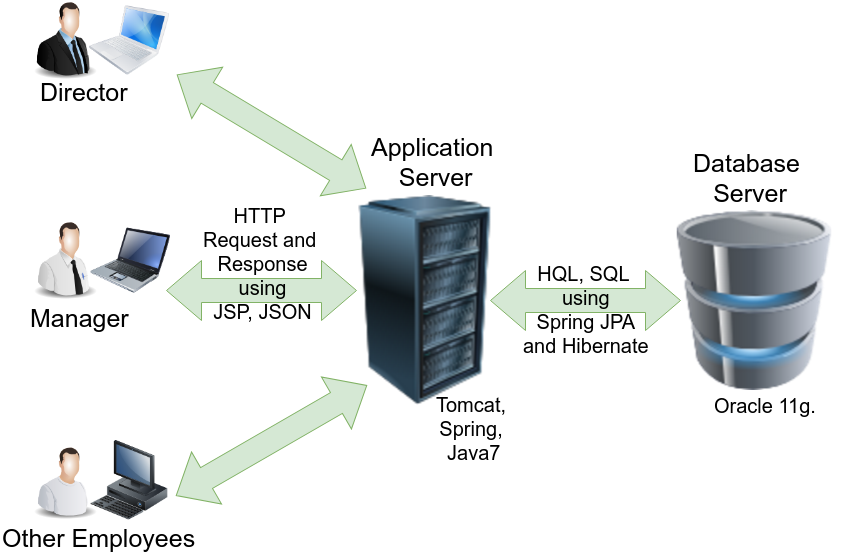
\includegraphics[width=\linewidth]{SML-AMS-System-Architecture.png}
    \caption{SML-AMS: System Architecture.}
    \label{fig:system-architecture}

\end{figure}

SML-AMS is an account and office management software which was developed for a sea port container handling and logistic company named Shafi Motors Limited\cite{SML:1965}. The system architecture is shown in Figure:~\ref{fig:system-architecture} where following technologies and tools were used:

\begin{itemize}

	\item JSP, Tiles, JSON were used to display data and interact with users.

	\item Middleware was developed using Spring Framework, Java7. To communicate with data storage, Spring JPA and Hibernate frameworks were used in the system.
    
    \item Jasper Report and JExcel API were used to generate vouchers, reports in pdf and excel formats.
    
    \item Application is running on Apache Tomcat server.
    
    \item For data storage, company's requirement was Oracle 11g.
    
    \item IntelliJ IDEA, Sql Developer were used as development tools.

\end{itemize}

The system has accounts, official and managerial modules. They are mentioned bellow in brief:

\begin{itemize}

	\item Admin: contains administrative and system level configurations such as user, role, group etc.
    
    \item Asset: using this module, company manages their assets.
    
    \item Transport: it is used for their logistic vehicles.
    
    \item Employee: this is a basic level HRM module.
    
    \item Requisition: company uses this module for any kind of requisition that is related to purchase.
    
    \item Expenditure: this module is for company expenditure.
    
    \item Purchase \& Invoice: this module is related to requisition and expenditure modules.
    
    \item Transaction: any kind of company money transactions are booked using this module.
    
    \item Bank Account: it is similar to company's bank account and is used for transaction related purpose for debit and credit amounts.
    
    \item Bill: the most important module of the system because using this module, company entry its monthly, yearly incomes and also calculates dues, VAT(Value Added Tax), Income Tax Return etc. 
    
    \item Reports: this module contains all system, asset and financial reports that can be downloaded as excel sheets.
    
\end{itemize}

\section{Unit Requirements}
\label{sec:unit-requirements}
Here in this report, the requirements of bill module is going to be discussed and later tested using test driven development approach. In bill module, user can work with 4 types of bills. They are:

\begin{itemize}
	
    \item Import: bills that are related to import materials from abroad.
    
    \item ICD: container handling bills.
    
    \item CFS: export materials related bills.
    
    \item Account: miscellaneous bills. 

\end{itemize}

The Table:~\ref{tab:requirements} describes the unit requirements of bill module by following Software Requirements Specifications(SRS)\cite{SRS:2010}. \\

\begin{center}
\begin{longtabu} to \linewidth {| l | X[2] | c |}
	
    \caption{SML-AMS: Requirements of Bill Module.}
    \label{tab:requirements} \\ 
  	\hline	
    \rowfont\bfseries Requirement ID & Requirement Statement & Priority \\ 
    \hline
    \endfirsthead
    
    \caption{SML-AMS: Requirements of Bill Module.} \\ 
    \hline	
    \rowfont\bfseries Requirement ID & Requirement Statement & Priority \\ 
    \hline 
    \endhead

    \multicolumn{3}{r}{} \\
    \multicolumn{3}{r}{(Please see in next page.)} \\
    \endfoot

    \endlastfoot

    \hline	
    SML-AMS-FR-1.0 & Create Import bills. & High \\
    \hline
    SML-AMS-FR-1.1 & Create VAT\--able Import bills. & High \\
    \hline
    SML-AMS-FR-1.2 & Create Non VAT\--able Import bills. & High \\
    \hline
    SML-AMS-FR-2.0 & Modify Import bills. & Normal \\
    \hline
    SML-AMS-FR-2.1 & Modify VAT\--able Import bills. & Normal \\
    \hline
    SML-AMS-FR-2.2 & Modify Non VAT\--able Import bills. & Normal \\
    \hline
    SML-AMS-FR-3.0 & Delete Import bills. & Low \\
    \hline
    SML-AMS-FR-3.1 & Delete VAT\--able Import bills. & Low \\
    \hline
    SML-AMS-FR-3.2 & Delete Non VAT\--able Import bills. & Low \\
    \hline
    SML-AMS-FR-4.0 & Create ICD bills. & High \\
    \hline
    SML-AMS-FR-4.1 & Create VAT\--able ICD bills. & High \\
    \hline
    SML-AMS-FR-4.2 & Create Non VAT\--able ICD bills. & High \\
    \hline
    SML-AMS-FR-5.0 & Modify ICD bills. & Normal \\
    \hline
    SML-AMS-FR-5.1 & Modify VAT\--able ICD bills. & Normal \\
    \hline
    SML-AMS-FR-5.2 & Modify Non VAT\--able ICD bills. & Normal \\
    \hline
    SML-AMS-FR-6.0 & Delete ICD bills. & Low \\
    \hline
    SML-AMS-FR-6.1 & Delete VAT\--able ICD bills. & Low \\
    \hline
    SML-AMS-FR-6.2 & Delete Non VAT\--able ICD bills. & Low \\
    \hline
    SML-AMS-FR-7.0 & Create CFS bills. & High \\
    \hline
    SML-AMS-FR-7.1 & Create VAT\--able CFS bills. & High \\
    \hline
    SML-AMS-FR-7.2 & Create Non VAT\--able CFS bills. & High \\
    \hline
    SML-AMS-FR-8.0 & Modify CFS bills. & Normal \\
    \hline
    SML-AMS-FR-8.1 & Modify VAT\--able CFS bills. & Normal \\
    \hline
    SML-AMS-FR-8.2 & Modify Non VAT\--able CFS bills. & Normal \\
    \hline
    SML-AMS-FR-9.0 & Delete CFS bills. & Low \\
    \hline
    SML-AMS-FR-9.1 & Delete VAT\--able CFS bills. & Low \\
    \hline
    SML-AMS-FR-9.2 & Delete Non VAT\--able CFS bills. & Low \\
    \hline
    SML-AMS-FR-10.0 & Create Account bills. & Low \\
    \hline
    SML-AMS-FR-10.1 & Create VAT\--able Account bills. & Low \\
    \hline
    SML-AMS-FR-10.2 & Create Non VAT\--able Account bills. & Low \\
    \hline
    SML-AMS-FR-11.0 & Modify Account bills. & Low \\
    \hline
    SML-AMS-FR-11.1 & Modify VAT\--able Account bills. & Low \\
    \hline
    SML-AMS-FR-11.2 & Modify Non VAT\--able Account bills. & Low \\
    \hline
    SML-AMS-FR-12.0 & Delete Account bills. & Low \\
    \hline
    SML-AMS-FR-12.1 & Delete VAT\--able Account bills. & Low \\
    \hline
    SML-AMS-FR-12.2 & Delete Non VAT\--able Account bills. & Low \\
    \hline
    SML-AMS-FR-13.0 & Approve any type of bills. & High \\
    \hline
    SML-AMS-FR-13.1 & User can not modify approved bills. & High \\
    \hline
    SML-AMS-FR-13.2 & User can not delete approved bills. & High \\
    \hline
    SML-AMS-FR-13.3 & User can not approve a approved bill again because it is already approved by someone else. & High \\
    \hline
    SML-AMS-FR-13.4 & User can not approve a received bill because it is already passed this step and after completion of bill receive, the life-cycle of a bill ends. & High \\
    \hline
    SML-AMS-FR-14.0 & Unapprove any type of bills. & High \\
    \hline
    SML-AMS-FR-14.1 & User can not unapprove a unapproved bill again because it is already unapproved by someone else. & High \\
    \hline
    SML-AMS-FR-14.2 & User can not unapprove a received bill because it is already passed this step and after completion of bill receive, the life-cycle of a bill ends. & High \\
    \hline
    SML-AMS-FR-15.0 & Create bill receive from bills that are added in system. & High \\
    \hline
    SML-AMS-FR-15.1 & A bill receive record must be for only one specific bill type. There is no possibility to exist one bill receive record for two or more bill types. & High \\
    \hline
    SML-AMS-FR-15.2 & A bill receive record must contains one or more bills of only one specific bill type. & High \\
    \hline
    SML-AMS-FR-15.3 & Bills within a bill receive record must be approved and not received yet(that means have due amount) & High \\
    \hline
    SML-AMS-FR-15.4 & Bill collection amount for each bill is always less than equal to bill amount. & High \\
    \hline
    SML-AMS-FR-15.5 & For each bill amount, user can add discount in flat or percentage format. & High \\
    \hline
    SML-AMS-FR-15.6 & For each bill amount, user can add deduction as Income Tax or TR(Treasury Challan) in flat or percentage format. & High \\
    \hline
    SML-AMS-FR-15.7 & Bill receive can be possible using cash or cheques or pay\--order or any combination. & High \\
    \hline
    SML-AMS-FR-15.8 & When total bill receivable amount and collected amount(by cash/cheque/pay\--order) is equal then this bill receive record should be auto completed by system. & High \\
    \hline
    SML-AMS-FR-15.9 & User can also mark a bill receive record as completed by manual process in the system. & Normal \\
    \hline
    SML-AMS-FR-15.10 & Maximum form fields(drop downs, text boxes, check boxes etc.) should be auto calculated(for amounts) and populated(for bills and amounts) by system. & High \\
    \hline
    SML-AMS-FR-15.11 & For amount values, no zero and negative values are allowed that means system should block each and every negative or zero values from user input or automatic calculation. & High \\
    \hline
    SML-AMS-FR-16.0 & Approve bill receive. & High \\
    \hline
    SML-AMS-FR-16.1 & User can not approve a approved bill receive record again because it is already approved by someone else. & High \\
    \hline
    SML-AMS-FR-16.2 & User can not approve a completed bill receive record. Completed bill receive record means when bill collection is done then a bill receive record is completed. & High \\
    \hline
    SML-AMS-FR-17.0 & Unapprove bill receive. & High \\
    \hline
    SML-AMS-FR-17.1 & User can not unapprove a unapproved bill receive record again because it is already unapproved by someone else. & High \\
    \hline
    SML-AMS-FR-17.2 & User can not unapprove a completed bill receive record. Completed bill receive record means when bill collection is done then a bill receive record is completed. & High \\
    \hline
    SML-AMS-FR-18.0 & Modify bill receive. & High \\
    \hline
    SML-AMS-FR-18.1 & User can not modify approved bill receive record. & High \\
    \hline
    SML-AMS-FR-18.2 & User can not modify completed bill receive record. Completed bill receive record means when bill collection is done then a bill receive record is completed. & High \\
    \hline
    SML-AMS-FR-19.0 & Delete bill receive. & Normal \\
    \hline
    SML-AMS-FR-19.1 & User can not delete approved bill receive record. & Normal \\
    \hline
    SML-AMS-FR-19.2 & User can not delete completed bill receive record. Completed bill receive record means when bill collection is done then a bill receive record is completed. & Normal \\
    \hline
    SML-AMS-FR-20.0 & User can not modify a received bill because it is already passed this step and after completion of bill receive, the life-cycle of a bill ends. & Normal \\
    \hline
    SML-AMS-FR-21.0 & User can not delete a received bill because it is already passed this step and after completion of bill receive, the life-cycle of a bill ends. & Normal \\
    \hline

\end{longtabu}
\end{center} 

\section{Test Strategy}
The main idea behind the general V-model is that development and testing tasks are corresponding activities of equal importance\cite{Spillner:Linz:Schaefer:2014}. The two branches of the V symbolize this. The left branch represents the development process. During development, the system is gradually being designed and finally programmed. The right branch represents the integration and testing process; the program elements are successively being assembled to form larger subsystems(integration), and their functionality is tested. Integration and testing end when the acceptance test of the entire system has been completed\cite{Spillner:Linz:Schaefer:2014}. \\

As per V-model, there are 4(four) level of testing in software development\cite{Spillner:Linz:Schaefer:2014}. They are as follows: 

\begin{itemize}
	
    \item Component Test: verifies whether each software component correctly fulfills its specification\cite{Spillner:Linz:Schaefer:2014}. 
    
    \item Integration Test: checks if groups of components interact in the way that is specified by the technical system design\cite{Spillner:Linz:Schaefer:2014}.
    
    \item System Test: verifies whether the system as a whole meets the specified requirements\cite{Spillner:Linz:Schaefer:2014}.
    
    \item Acceptance Test: checks if the system meets the customer requirements, as specified in the contract and/or if the system meets user needs and expectations\cite{Spillner:Linz:Schaefer:2014}. \\

\end{itemize} 

The current status of the application is active and running on company's\cite{SML:1965} internal server. Company is properly and actively using this system since 2015 for its accounts and office management purposes. During software module and phase development, many static tests were done by both developers and company's IT professionals. So here "Integration Test"\cite{Spillner:Linz:Schaefer:2014}, "System Test"\cite{Spillner:Linz:Schaefer:2014} and "Acceptance Test"\cite{Spillner:Linz:Schaefer:2014} are not necessary. \\ \\ 
For this test reporting purpose, the "Reactive Test Strategy"\cite{Spillner:Linz:Schaefer:2014} is going to be used. Under this test strategy, it is going to create some "Component Test" cases from the unit requirements~\ref{tab:requirements} that are described in previous section~\ref{sec:unit-requirements} using a well known and popular test design method named "State Transition Testing"\cite{Spillner:Linz:Schaefer:2014} technique. Here Figure:~\ref{fig:bill-fsm-diagram} shows the state transition diagram of a company's bill that are recorded in the system. In addition, Figure:~\ref{fig:bill-transition-tree} displays the transition tree for test cases. From these both diagrams, it is seen that there are two finishing states for this bill state transition diagram. The two final states are "Received" and "Deleted" respectively. 

\begin{figure}

	\centering
    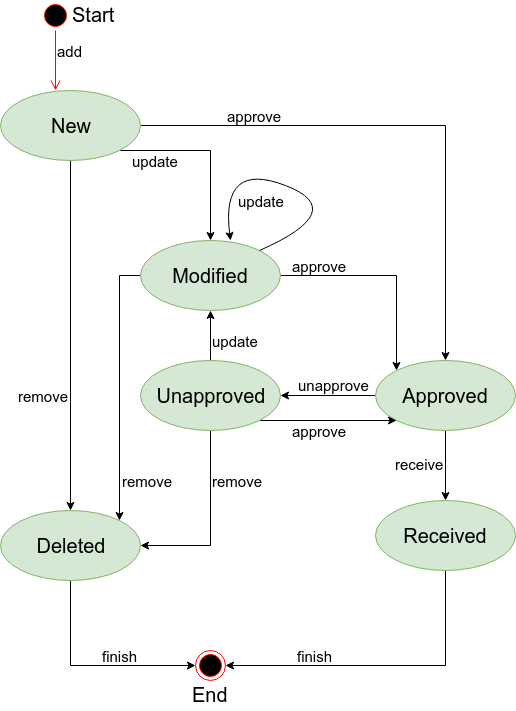
\includegraphics[scale=0.7]{SML-AMS-Bill-FSM-Diagram.png}
    \caption{SML-AMS: Bill Finite State Machine(FSM) Diagram.}
    \label{fig:bill-fsm-diagram}

\end{figure}

\begin{figure}

	\centering
    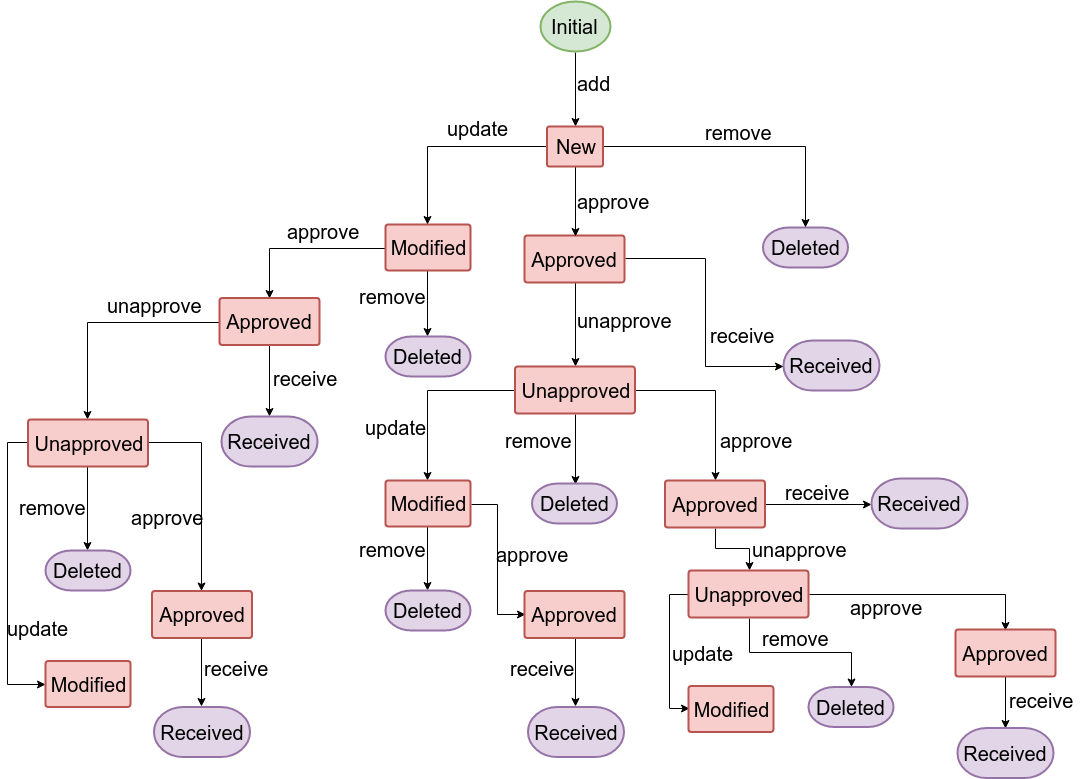
\includegraphics[scale=0.395]{SML-AMS-Bill-Transition-Tree.png}
    \caption{SML-AMS: Bill Transition Tree for test cases.}
    \label{fig:bill-transition-tree}

\end{figure}

\newpage

\section{Dynamic Test Cases}
It is planned to do some component level dynamic tests that are under back box testing category. The justification behind the selection of the test design methods, test cases, risk analysis and test end criteria are given bellow: 

\subsection{Goal}
Add a VAT\--able Import bill from scratch that means before add operation, this to-be bill has no existence in the system. Then update that bill. After that approve the bill and finally receive bill amount from client. Beside these sequences, it is planned to test other transition sequences from Bill Finite State Machine(FSM) and Transition Tree diagrams that are given in Figure:~\ref{fig:bill-fsm-diagram} and Figure:~\ref{fig:bill-transition-tree} respectively.  

\subsection{Design Method}
From the above goal statement, it is seen that there are is an initial state named "Initial", expected behaviors named "add", "update", "approve", "unapprove", "receive", "remove" and expected final states named "Received", "Deleted". So the "State Transition Testing" technique is planned to use for doing these dynamic component tests.

\subsection{Risk Analysis}
Some key points on possible risk factors are given bellow:

\begin{itemize}

	\item Have chance to break the transition sequences. 
    
    \item Programming syntax errors in test codes.
    
    \item Wrong use of mock up objects.
    
    \item Internal logic errors inside component or classes or methods.

\end{itemize}

\subsection{Test End Criteria}
End criteria for dynamic compontent test cases are mentioned bellow\cite{Spillner:Linz:Schaefer:2014}:

\begin{itemize}
	
    \item Every states has been reached at least once according transition sequence.
    
    \item Test case must have a start state and an end/finish state.
    
    \item Every transition has been executed at least once.\cite{Spillner:Linz:Schaefer:2014}

\end{itemize}

\subsection{Input Data}
Possible input data for dynamic component test cases are:

\begin{itemize}

	\item A VAT\--able Import Bill.
    
    \item A non VAT\--able Import Bill.
    
    \item A VAT\--able ICD Bill.
    
    \item A non VAT\--able ICD Bill.
    
    \item A VAT\--able CFS Bill.
    
    \item A non VAT\--able CFS Bill.

\end{itemize}

\subsection{Test Cases}
The Table:~\ref{tab:dynamic-test-cases} that is drawn in bellow, represents the test cases with proper and related references to unit requirements~\ref{sec:unit-requirements} that are mentioned in Table:~\ref{tab:requirements}. \\

\begin{center}
\begin{longtabu} to \linewidth {| X[1] | X[2] | c |}
	
    \caption{SML-AMS: Dynamic Component Test Cases.}
    \label{tab:dynamic-test-cases} \\ 
  	\hline	
    \rowfont\bfseries Reference & Test Case & Priority \\ 
    \hline
    \endfirsthead
    
    \caption{SML-AMS: Dynamic Component Test Cases.} \\ 
    \hline	
    \rowfont\bfseries Reference & Test Case & Priority \\ 
    \hline 
    \endhead

    \multicolumn{3}{r}{} \\
    \multicolumn{3}{r}{(Please see in next page.)} \\
    \endfoot

    \endlastfoot

    \hline	
    SML-AMS-FR-1.1, SML-AMS-FR-2.1, SML-AMS-FR-13.0, SML-AMS-FR-15.8 & initialize(Initial), add(New), update(Modified), approve(Approved), receive(Received). & High \\
    \hline
	SML-AMS-FR-4.1, SML-AMS-FR-6.1 & initialize(Initial), add(New), remove(Deleted). & Normal \\
    \hline
	SML-AMS-FR-1.2, SML-AMS-FR-13.0, SML-AMS-FR-15.8 & initialize(Initial), add(New), approve(Approved), receive(Received). & High \\
    \hline
	SML-AMS-FR-7.2, SML-AMS-FR-9.2, SML-AMS-FR-13.0, SML-AMS-FR-14.0 & initialize(Initial), add(New), approve(Approved), unapprove(Unapproved), remove(Deleted). & High \\
    \hline
	SML-AMS-FR-1.1, SML-AMS-FR-2.1, SML-AMS-FR-3.1 & initialize(Initial), add(New), update(Modified), remove(Deleted). & Normal \\
    \hline
	SML-AMS-FR-1.2, SML-AMS-FR-2.2, SML-AMS-FR-13.0, SML-AMS-FR-14.0, SML-AMS-FR-15.8 & initialize(Initial), add(New), approve(Approved), unapprove(Unapproved), update(Modified), approve(Approved), receive(Received). & High \\
    \hline
    SML-AMS-FR-7.1, SML-AMS-FR-8.1, SML-AMS-FR-9.1, SML-AMS-FR-13.0, SML-AMS-FR-14.0 & initialize(Initial), add(New), approve(Approved), unapprove(Unapproved), update(Modified), remove(Deleted). & Normal \\
    \hline
    SML-AMS-FR-4.1, SML-AMS-FR-5.1, SML-AMS-FR-13.0, SML-AMS-FR-14.0, SML-AMS-FR-15.8 & initialize(Initial), add(New), update(Modified), approve(Approved), unapprove(Unapproved), update(Modified), approve(Approved), receive(Received). & High \\
    \hline 
    SML-AMS-FR-1.1, SML-AMS-FR-2.1, SML-AMS-FR-3.1, SML-AMS-FR-13.0, SML-AMS-FR-14.0 & initialize(Initial), add(New), update(Modified), approve(Approved), unapprove(Unapproved), remove(Deleted). & Normal \\
    \hline
  	SML-AMS-FR-7.2, SML-AMS-FR-8.2, SML-AMS-FR-9.2, SML-AMS-FR-13.0, SML-AMS-FR-14.0 & initialize(Initial), add(New), update(Modified), approve(Approved), unapprove(Unapproved), update(Modified), remove(Deleted). & High \\  
    \hline
    
\end{longtabu}
\end{center}

\section{Static Testing}
Company is properly and actively using this system since 2015 for its accounts and office management purposes. During software module and phase development, many static tests were done by both developers and company's IT professionals. So here static testing is not necessary and the report is written based on component level test cases of bill module.  

\section{My Experience}
From this course and test report, the learned topics and experiences are summarized bellow: %in Table:~\ref{tab:experience-summary}.

\begin{itemize}
	
    \item Exercise Number: 01.
    
    \item Date: \thedate.

	\item Title of Exercise: Create and test some Component Test Cases using State Transition test design technique.
    
    \item Description: Test cases that are mentioned in the Table: ~\ref{tab:dynamic-test-cases}, are component level test cases of bill module. These cases are created from two figures \--- Figure:~\ref{fig:bill-fsm-diagram} and Figure:~\ref{fig:bill-transition-tree} respectively. Tests are programmed using Java, JUnit, Mockito. The test cases cover almost every state transitions of a bill within bill module of SML-AMS application.
    
    \item Results: All tests are passed successfully as the system is already running and bill module is the main important module of the system. During the developments, static tests were done to check these state transitions. But now with the help of this dynamic component testing, all state transitions are automatically checked and tested which make the module more solid and error free.

	\item I learn how to think and plan to create test cases of a software module before implementation using general V-model, black box testing, white box testing and other test design techniques. Here I especially learn on State Transition Testing technique by making Finite State Machine(FSM) diagram and Transition Tree that are totally new for me in testing ground. I also learn about LaTeX which is really a powerful and excellent writing tools I have ever seen. 

	\item Author: \theauthor 
    
    \item Date: \thedate
    
\end{itemize}


%\begin{center}
%\begin{longtabu} to \linewidth {| l | X[2] |}
	
%    \caption{SML-AMS: Summary of Achieved Experiences.}
%    \label{tab:experience-summary} \\ 
%  	\hline
%    \endfirsthead
    
%    \caption{SML-AMS: Summary of Achieved Experiences.} \\ 
%    \hline 
%    \endhead

%    \multicolumn{2}{r}{} \\
%    \multicolumn{2}{r}{(Please see in next page.)} \\
%    \endfoot

%    \endlastfoot

%    \hline	
%    Exercise Number: 01 & Date: \thedate \\
%    \hline
%    \multicolumn{2}{l}{Title of Exercise: Create and test some Component Test Cases using State Transition test design technique.} \\  
%	\hline
%    \multicolumn{2}{l}{Description: Test cases that are mentioned in the Table: ~\ref{tab:dynamic-test-cases}, are component level test cases of bill module. These cases are created from two figures \--- Figure:~\ref{fig:bill-fsm-diagram} and Figure:~\ref{fig:bill-transition-tree} respectively. Tests are programmed using Java, JUnit, Mockito. The test cases cover almost every state transitions of a bill within bill module of SML-AMS application.} \\
%	\hline
%    \multicolumn{2}{l}{Results: All tests are passed successfully as the system is already running and bill module is the main important module of the system. During the developments, static tests were done to check these state transitions. But now with the help of this dynamic component testing, all state transitions are automatically checked and tested which saves not only time but also } \\
%	\hline
%    \multicolumn{2}{l}{What did you learn?} \\
%	\hline
%    Author: \theauthor & Date: \thedate \\ 
%	\hline
    
%\end{longtabu}
%\end{center}

\newpage

\section{Sample Codes}
\begin{lstlisting}
@Test
	public void testVatableImportBill_New_Modified_Approved_Received() {
		
		when(billService.saveBill(Bill.class)).thenReturn(mockImportBill);
		when(billReceiveService.saveBillReceiveWithAssociations(BillReceive.class))
        .thenReturn(mockImportBill);	
		
		assertEquals("Import Bill is not in 'Initial' state", null, importBill.getId());
		
		Bill bill = billService.saveBill(importBill);

		assertEquals("Import Bill is not in 'New' state", newImportBill.getId(), bill.getId());

		mockImportBill.setVersion(5);
		bill = billService.saveBill(importBill);

		assertTrue("Import Bill is not in 'Modified' state", bill.getVersion() > importBill.getVersion());
		
		// import bill is not in approved state so next state will be approved state
		assertEquals("Import Bill is in 'Approved' state", null, bill.getApprovedBy());

		mockImportBill.setApprovedBy(new User(1001, 0, "test_user_123"));
		mockImportBill.setReceived(Boolean.FALSE);
		
		bill = billService.saveBill(importBill);
				
		assertEquals("Import Bill is not in 'Approved' state", mockImportBill.getApprovedBy(), bill.getApprovedBy());

		// import bill is not in received state so next state will be received state
		assertEquals("Import Bill is in 'Received' state", Boolean.FALSE, bill.getReceived());
		
		mockImportBill.setReceived(Boolean.TRUE);
		
		bill = billReceiveService.saveBillReceiveWithAssociations(billRecieveObj);

		assertEquals("Import Bill is not in 'Received' state", Boolean.TRUE, bill.getReceived());
	}
\end{lstlisting}

\section{Alle Test Cases}
The details test cases from Table:~\ref{tab:dynamic-test-cases} are described bellow:

\subsection{Test 01}
\begin{itemize}
	
    \item ID: BillControllerTest-01.
    
    \item Title: testVatableImportBill\_New\_Modified\_Approved\_Received.
    
    \item Author: \theauthor.
    
    \item Input Data: a mock Import Bill which is VAT-able. This Import bill object has no object id that means it is in initial state.
    
    \item Expected Outcome: an Import Bill having object id and "received" boolean flag true which will indicate that bill's final state will "Received" as per State Transition Testing technique(Figure:~\ref{fig:bill-fsm-diagram}).
    
    \item Actual Outcome: mock Import Bill has object id and also "received" boolean flag is true.
    
    \item Result: Passed.

\end{itemize}

\subsection{Test 02}
\begin{itemize}
	
    \item ID: BillControllerTest-02.
    
    \item Title: testVatableICDBill\_New\_Deleted.
    
    \item Author: \theauthor.
    
    \item Input Data: a mock ICD Bill which is VAT-able. This ICD bill object has no object id that means it is in initial state.
    
    \item Expected Outcome: an ICD Bill having object id and removed from system which will indicate that bill's final state will "Deleted" as per State Transition Testing technique(Figure:~\ref{fig:bill-fsm-diagram}).
    
    \item Actual Outcome: mock Import Bill has object id and also "Deleted" from system.
    
    \item Result: Passed.

\end{itemize}

\subsection{Test 03}
\begin{itemize}
	
    \item ID: BillControllerTest-03.
    
    \item Title: testNonVatableImportBill\_New\_Approved\_Received.
    
    \item Author: \theauthor.
    
    \item Input Data: a mock Import Bill which is non VAT-able. This Import bill object has no object id that means it is in initial state.
    
    \item Expected Outcome: an Import Bill having object id and "received" boolean flag true which will indicate that bill's final state will "Received" as per State Transition Testing technique(Figure:~\ref{fig:bill-fsm-diagram}).
    
    \item Actual Outcome: mock Import Bill has object id and also "received" boolean flag is true.
    
    \item Result: Passed.

\end{itemize}

\subsection{Test 04}
\begin{itemize}
	
    \item ID: BillControllerTest-04.
    
    \item Title: testNonVatableCFSBill\_New\_Approved\_Unapproved\_Deleted.
    
    \item Author: \theauthor.
    
    \item Input Data: a mock CFS Bill which is non VAT-able. This CFS bill object has no object id that means it is in initial state.
    
    \item Expected Outcome: an CFS Bill having object id and removed from the system which will indicate that bill's final state will "Deleted" as per State Transition Testing technique(Figure:~\ref{fig:bill-fsm-diagram}).
    
    \item Actual Outcome: mock CFS Bill has object id and also removed from the system.
    
    \item Result: Passed.

\end{itemize}

\subsection{Test 05}
\begin{itemize}
	
    \item ID: BillControllerTest-05.
    
    \item Title: testVatableImportBill\_New\_Modified\_Deleted.
    
    \item Author: \theauthor.
    
    \item Input Data: a mock Import Bill which is VAT-able. This Import bill object has no object id that means it is in initial state.
    
    \item Expected Outcome: an Import Bill having object id and removed from the system which will indicate that bill's final state will "Deleted" as per State Transition Testing technique(Figure:~\ref{fig:bill-fsm-diagram}).
    
    \item Actual Outcome: mock Import Bill has object id and also removed from the system.
    
    \item Result: Passed.

\end{itemize}

\subsection{Test 06}
\begin{itemize}
	
    \item ID: BillControllerTest-06.
    
    \item Title: testNonVatableImportBill\_New\_Approved\_Unapproved\_Modified\_Approved\_Received.
    
    \item Author: \theauthor.
    
    \item Input Data: a mock Import Bill which is non VAT-able. This Import bill object has no object id that means it is in initial state.
    
    \item Expected Outcome: an Import Bill having object id and "received" boolean flag true which will indicate that bill's final state will "Received" as per State Transition Testing technique(Figure:~\ref{fig:bill-fsm-diagram}).
    
    \item Actual Outcome: mock Import Bill has object id and also "received" boolean flag is true.
    
    \item Result: Passed.

\end{itemize}

\subsection{Test 07}
\begin{itemize}
	
    \item ID: BillControllerTest-07.
    
    \item Title: testVatableCFSBill\_New\_Approved\_Unapproved\_Modified\_Deleted.
    
    \item Author: \theauthor.
    
    \item Input Data: a mock CFS Bill which is VAT-able. This CFS bill object has no object id that means it is in initial state.
    
    \item Expected Outcome: an CFS Bill having object id and removed from the system which will indicate that bill's final state will "Deleted" as per State Transition Testing technique(Figure:~\ref{fig:bill-fsm-diagram}).
    
    \item Actual Outcome: mock CFS Bill has object id and also removed from the system.
    
    \item Result: Passed.

\end{itemize}

\subsection{Test 08}
\begin{itemize}
	
    \item ID: BillControllerTest-08.
    
    \item Title: testVatableICDBill\_New\_Modified\_Approved\_Unapproved\_Modified\_Approved\_Received.
    
    \item Author: \theauthor.
    
    \item Input Data: a mock ICD Bill which is VAT-able. This ICD bill object has no object id that means it is in initial state.
    
    \item Expected Outcome: an ICD Bill having object id and "received" boolean flag true which will indicate that bill's final state will "Received" as per State Transition Testing technique(Figure:~\ref{fig:bill-fsm-diagram}).
    
    \item Actual Outcome: mock ICD Bill has object id and also "received" boolean flag is true.
    
    \item Result: Passed.

\end{itemize}

\subsection{Test 09}
\begin{itemize}
	
    \item ID: BillControllerTest-09.
    
    \item Title: testVatableImportBill\_New\_Modified\_Approved\_Unapproved\_Deleted.
    
    \item Author: \theauthor.
    
    \item Input Data: a mock Import Bill which is VAT-able. This Import bill object has no object id that means it is in initial state.
    
    \item Expected Outcome: an Import Bill having object id and removed from the system which will indicate that bill's final state will "Deleted" as per State Transition Testing technique(Figure:~\ref{fig:bill-fsm-diagram}).
    
    \item Actual Outcome: mock Import Bill has object id and also removed from the system.
    
    \item Result: Passed.

\end{itemize}

\subsection{Test 10}
\begin{itemize}
	
    \item ID: BillControllerTest-10.
    
    \item Title: testNonVatableCFSBill\_New\_Modified\_Approved\_Unapproved\_Modified\_Deleted.
    
    \item Author: \theauthor.
    
    \item Input Data: a mock CFS Bill which is non VAT-able. This CFS bill object has no object id that means it is in initial state.
    
    \item Expected Outcome: an CFS Bill having object id and removed from the system which will indicate that bill's final state will "Deleted" as per State Transition Testing technique(Figure:~\ref{fig:bill-fsm-diagram}).
    
    \item Actual Outcome: mock CFS Bill has object id and also removed from the system.
    
    \item Result: Passed.

\end{itemize}

\newpage

\appendix
\section{Appendix}
\listoffigures
\listoftables

\newpage

\bibliographystyle{plain}
\bibliography{biblist}

\end{document}